\chapter{Simulation}
\label{simulation}
\epigraph{A model is a physical, mathematical, or logical representation of a system entity, phenomenon, or process. 
A simulation is the implementation of a model over time. 
A simulation brings a model to life and shows how a particular object or phenomenon will behave.}
{\textit{Systems Engineering Fundamentals. Defense Acquisition University Press, 2001}}

{}To evaluate various strategies when evolving a component system, the environment in which these evolutions occur must be studied.
{}This study can be in the form of either looking at real systems and users, studying a system in a controlled environment or simulating the environment in an abstract manner.
{}Each of these options is discussed and weighed for their costs and benefits.
{}The simulation method is selected as it has the best attributes required for this research.

{}The methodology that \cite{Law2005} outlines is used to create a valid and credible simulation.
{}The basic artifact of this methodology is a ``conceptual model'', this is an simplified abstraction of reality.
{}It describes the individual sub-models of the user, repository, and resolver; the variables in the configuration of the simulation;
{}and the processes in which these variables are used to simulate reality.
{}This chapter concludes with the discussion of the validation process of this conceptual model.

\section{Problem Definition}
The problem addressed in this thesis is outlined by the thesis question (previously defined in chapter \ref{introduction},

\begin{quotation}
``What effect does using component dependency resolution with different strategies have on system evolution?''
\end{quotation}

Component system evolution, component dependency resolution and evolution strategies have been reviewed in their respective previous chapters \ref{background}, \ref{cdr} and \ref{strategies}.
To solve this problem, the effects being measured must be further defined.

%%%The most important effects are related to the objective of the strategy
The effects that are most closely studied are those that are a measurement of how effectively a strategy satisfies its objectives.
For example, if a server administrator uses a particular strategy in order to be up to date with minimum change,
the measurement of how up to date their system is per change made is an important effect to be measured.

%%%There is also side effect, what unintended consequences occur because of the use of a strategy
Other effects of the strategy are also important to measure.
The unintended consequences, side effects, of using a strategy can be important as well.
A given strategy may fulfill all its objectives, though degrade the system by some other measure.
For example, the server administrators strategy may keep a system up to date with little change, 
though it may increase internal complexity of the system making it unstable. 

\section{How to Answer the Thesis Question}
%%%What we need to have to answer the question? A time line of systems created using different strategies.
To study the effects of different strategies on component system evolution requires the study of the systems and how they change over a period of time given the strategy employed. 
Each system along this evolutionary timeline can be studied and analysed for the effects of the strategy.
For any given strategy multiple different samples of timelines must be collected as different factors create a range of possible outcomes of any strategy.
These strategies can then be compared by the effects that are caused to the system.

%%%How to get this timeline of systems
To get this timeline of systems, real systems and users could be used and actual field data collected;
a controlled environment could be created, where users employ strategies on a system that is monitored;
or a simulation of a systems evolution is created, where different aspects are modelled and processed by an algorithm to generate the systems.
In this section the positive and negative aspects of each of these approaches are discussed,
and the reasons for the selection of the simulation method for this research are presented.

\subsection{Using Real Users and Systems}
%%%The pros and cons of using real systems with real users
Using real systems with real users would produce real and valid data to analyse evolution strategies.
Users could be recruited to employ different strategies on their actual systems, while software monitoring their system would collect data.
Resolvers with strategy specific criteria would also have to be developed and distributed to the users.
After a period of time the information of the systems evolution could be retrieved and analysed.

%%%Now the cons %How about incomparible users/ if they use different systems from differntn starting points will haveto be handeled
This approach will create valid results, as the data would be real making the validity easily accessed. 
However, it has significant drawbacks,
it will take long periods of time to create meaningful results, for each day of results a day has to pass.
The most difficult hurdle will be finding users that will trust an experimental resolver to alter their real system.   
As even the slightest error from a resolver can cause a system to become unstable, a user will likely not trust a resolver without a significant amount of validation.

%%%Users trust is difficult to gain
To gain the trust of possible users the experimental resolvers would have to be thoroughly tested through a managed development cycle and be well maintained.
Moving a component through this cycle can be itself a massive undertaking lasting several months. 
For example, the development of Eclipse Plug-ins involves a component going through four phases 
Proposal, Incubation, Mature, and Top-Level \cite{eclipseDevelmonetProject};
similar to Debian's process of moving through the phases Unstable, Testing, Frozen, and finally stable \cite{Barth2005}.
After it has been through this cycle, maintenance of the resolver will likely be required.
This shows how much effort must be applied to earn a users trust, and this effort will likely outweigh the actual benefits.

\subsection{Users in a Controlled Environment}
%%%The pros and cons of using real users with pseduo systems
To increase the efficiency of collecting results a study of users interacting with a system in a monitored and controlled environment could be executed.
Each user could be given different strategies and different tasks to perform on their system to approximate real interactions.

This study could compress a years worth of interactions with a system into an hour, and produce results from real users. 
This research also removes the necessity of user trust as the user is altering a system that is not theirs.
However, it will also produce less valid results, as it is still an approximation of a real system, and the users know this.
Any controlled environment would alter how the user interacts with their controlled system, making the results less reliable.
For example, a user typically researches a component before selecting installing it because it would have real implications, 
in a controlled environment these implications are removed so the selection would still be of questionable validity.

However, the largest problem with this method is the effort required to conduct the experiment on enough users to find significant results.
Each user must be found and organised into a location for them to be monitored using a system.
The resources necessary to organise the amount of necessary users may exceed the resources of this study.
For example, given 10 different strategies want to be tested each 30 times to find statistically significant results, 
if an individual subject takes upwards of an hour to complete the study.
This would be 300 hours of effort, not including the organisation and preparation going into the study.

\subsection{Simulating the Problem}
%%%Instead we can simulate, with an approximation of the real world.\\ 
%%%When drawing conclusions the accuracy of this approximation must be considered, therefore significant effort has gone into data collection and validation.
A simulation is a surrogate of the real system, 
such that it represents the core aspects of the reality while simplifying and abstracting away unnecessary detail.
This is accomplished through modelling the most important parts of the system, 
and computationally creating and measuring the results. 
The goal of a simulation is not to represent every aspect of the real world, 
but to make a ``close enough'' approximation so that the conclusions drawn from it are valid while minimising complexity.

When analysing the results and forming conclusions from a simulation, 
the assumptions and abstractions made, must be taken into account. %TODO ref
Therefore, the majority of the effort when creating a simulation is defining the problem in such a way that the reality is simplified, but not over simplified.

\subsection{Why Simulate?}
%%%What is good about the simulation over the other two methods, speed at which results are generated, the cost to get the results, the control over the variables in the simulation.
The advantages of simulating are the speed at which ideas can be tested and evaluated;
the cost to test and get results; and the control over variables and configuration of the environment.

%%%Speed at which results are generated
The core steps to generate new knowledge is the iterative process of having an idea for a possible solution to a problem; 
testing it to find why, or why not, it is applicable to the problem;
and then forming new ideas based on the original for further study.
As the speed of this process increases, the greater amount of knowledge and meaningful information that can be generated. 
Using real users, or real systems, requires long periods of waiting and preparation where little or no progress is made.
However, if the actions and environment can be modeled and executed computationally, these times of no progress are eliminated.
Through simulation multiple ideas can simultaneously be tested almost immediately after they have been defined.
The same cannot be said for using real users or systems, where the turn around could be days or months to generate the same results.  

%%%Cost
The cost of getting the necessary results can be measured in the amount of time it would take in organising, measuring and wasted time, for the the results to be collected.
Using a real user and system would involve an enormous amount of time validating and distributing the solvers (as discussed earlier), 
and the controlled environment would require many hours of organisation and planning to gather the necessary users, and then measuring their interactions with the system.
However, with a simulation the main effort is ensuring that the models are accurate enough to gather meaningful results.
This time in validating the simulation and associated models is only necessary once, 
i.e. if more results are needed the simulation will not need to be re-validated.

%%%Control
The control over the results that a simulation returns far exceeds the other methods as models can be altered and tested where a real user cannot. 
This control allows the testing of extreme situations, the sensitivity analysis of different variables,
and the generation of possibly optimal but `out of the box' ideas. 
For instance, when finding an optimal update probability for a user, a range of values can be simulated and analysed.
If real users were used, the amount of users necessary to be found would be enormous to produce any significant results in this area.

%%%Final words on why we simulate
A simulation was used as it provides us with a cost/benefit ratio that is desirable, while potentially allowing an appropriate level of accuracy to draw meaningful conclusions.
The main effort was towards creating the simulation with valid models for the desired accuracy of this research.

\section{Methodology}
%%%We use the methodology from `` Build a Valid and Credible Simulation''
{}The core hurdle in using a simulation is validating the results and conclusions, and assuring their credibility.
{}This places validity and credibility of a simulation and the results it provides at a high priority.
{}To create a valid and credible simulation the methodology that \cite{Law2005} outlines is followed.
{}This methodology is a guideline for defining the study, collecting information, creating and validating models, and running the simulation.

This methodology has been used in numerous contexts. %TODO

{}In this section the methodology is described and aligned to this study's stated objectives. 
{}The steps that it states should be taken to create a valid simulation, and how the simulation will be created and what it will produce for this study are then discussed.

\subsection{Validation and Credibility}
%%%Why do we use this methodology and how is it relevant?
This methodology was created after the observation that validation was often ``attempted after the simulation models had already been developed'' \cite{Law2005}.
That is even if validation was attempted, it may only occurred if there was money and time left at the end of the project.
However, such simulations, that are not validated, can produce erroneous information that leads to bad, possibly costly decisions being made.
This reduces the credibility of the simulation to be used in future as a tool.

%%%What is a valid simulation?
A simulation is an abstraction and simplification of reality, often created as using an actual system can be disruptive, not cost-effective, or simply impossible.
In this context,

\begin{quotation}
``\textit{Validation} is the process of determining whether a simulation is an accurate representation of the system, for the particular object of the study.'' \cite{Law2005}
\end{quotation}

The latter part is an important aspect of validation, as the accuracy of the simulation is directly dependent on the problem and questions the study addresses.
Therefore, the definition of the problem will directly lead to the modelling and scope of the simulation.

%%%What is credible
A simulation, and by extension its results, have \textit{credibility} if key stakeholders accept them as ``correct''.
A credible model is not necessarily valid, and vice-versa, as it involves the input of a person who decides if the goals of the simulation have been obtained.
Credibility of a simulation is then only attainable if the key personale from the project understand and are involved directly with the project.

The simulation produced by this study to identify the effect of different strategies on the evolution of component systems must be validated to produce meaningful results,
and must be credible for these results to be trusted.

\subsection{Seven Step Method}
The methodology presented in \cite{Law2005} has a seven step approach to creating a valid and credible simulation.
These steps are; formulating the problem; collecting information and data to construct a conceptual model; validating the conceptual model;
implementing (programming) the model; validating the programmed model; designing, conducting and analysing experiments; and documenting and presenting the simulation results.

\subsubsection{Step 1: Formulate the problem}
The first step is to formulate the problem as clearly as possible, this is usually done with core stakeholders in a ``kick-off meeting''.
The core artifacts from this step are the overall objectives of the study, specific questions wanting to be answered, scope of the study,
 and different configurations of the simulation with the measures used to evaluate their performance. 

\subsubsection{Step 2: Collect information and data to construct conceptual model}
The conceptual model is a description of how the simulation and system work relative to the problems earlier defined.
It is the most important artifact of the simulation.
It should be high level enough to be understood by the core stakeholders but detailed enough to be reused in future simulations.
It is created through interviews with subject matter experts and collecting relevant data like results from similar exiting systems.
Problems like the data not being representative of the model, not being in the appropriate format or type, and containing errors must be handled before use.

The conceptual model also contains all of the variables that can be configured including their documented assumptions. 
It is defined to the level of detail with respect to project objectives, performance measures, data availability, computer constraints, and resource constraints.

\subsubsection{Step 3: Conceptual model validation}
The conceptual model is the most important aspect of the simulation, thus its validation must be thorough.
The core method used to validate this model, is to discuss it with core-stakeholders and subject matter experts.
This provides feedback as to the direction of the conceptual model, ensuring that it will answer the questions posed in the study.

\subsubsection{Step 4: Implement the conceptual model}
The implementation of the conceptual model must also be executed and documented in a way that allows others to replicate and repeat the process.
The artifacts created during this process must be verified to work correctly, this can be accomplished through test-cases and debugging \cite{Pressman1992}.

\subsubsection{Step 5: Validate implementation}
There is no completely definitive approach to validating the simulation,
however, the most definitive test of a simulations validity is established by closely looking at the outputted results compared to that from an actual system \cite{Law2005}.

This is done through:
\begin{itemize}
  \item \textbf{Results validation: } a comparable system is used to create results and compared with the results from the simulation for validation.
  \item \textbf{Face Validation: } experts are given output of the simulation model and checked to see if it is consistent with how they perceive the system should operate.
\end{itemize}

Further validation of the implementation can be accomplished with sensitivity analysis,
which is performed on the simulation to find the factors with the greatest impact on the performance and results.

\subsubsection{Step 6: Design, conduct and analyse experiments}
For each of the experiments that are run, the time and number of independent runs must be defined.
If the results are inconclusive, or other aspects of interest have arisen, it may be necessary to run additional experiments.

\subsubsection{Step 7: Document and present results}
This step involves the presentation of the conceptual model, simulation, and results to the core-stakeholders.
This presentation is critical for the future re-use of the model, as it should promote credibility through describing the validation process.

\subsection{Differences in methodology}
A core goal of creating this simulation study is to produce valid and credible results.
However, this specific methodology has been created for large scale industrial projects with substantial resources.
As this study is smaller in scale and resources some of the procedures recommended in this methodology have been restricted and some removed.

The most significant difference between this study and the described methodology is the clear definition between decision-maker and simulation designer.
In larger projects a simulation designer is contracted by a person who has a problem to solve or question to answer, a decision-maker.
In this project both these people are the same person, therefore meetings between them are not required.

Other people in the project including subject-matter experts, core-stakeholders, simulation analysts consist of survey participants and
project supervisors.
This is because the limits of the projects resources excludes the employment of experts for validation.
This may reduce the validity of the end model, but these restrictions have been made when only necessary,
and done so in a manner that attempts to minimise negative effects.

\subsection{Alternate methodologies}
%%%TODO
\section{Conceptual Model}
In this section the ``conceptual model'' of the process of component evolution using component dependency resolution.
This model describes the core elements of involved in this evolution, as well as the interactions between them.
The goal of the conceptual model is not to specify concrete values to the simulation, 
but as an abstract description that can be configured to ultimately answer the thesis question.

In this section, the three sub-models, the user model, the resolver model, and the repository model that make up the conceptual model are discussed.
These models contain variables that configure the simulation to represent various environments.
The processes used to simulate are also part of this conceptual model, and how they use the configuration to simulate component evolution is described. 

\subsection{User Model}
%%%The user can in reality execute many actions
A user can execute many different actions to alter their system like installing, removing or upgrading a component.
Also upgrading the entire system, downloading a source for a component, changing the status of a component, 
automatically removing components that are not necessary, or even formatting the system and starting again.
The possible list of actions is massive to provide the user with many different options in which to accomplish various tasks.
However, many of these actions are only used in niche cases, and are not typically used.

%%%We have limited it to two actions, install and update, as they are the core actions a user executes
In our simulation the user has two actions to alter their systems; either to install a new component or to upgrade the entire system.
These two action were selected as they represent the core interactions the user performs on the system.
The probability of these actions being taken, and also the parameters of an action must also be included in this model.

The initial system the user installs is also modelled here, as this is the starting point of any evolution.

%%%Update
\subsubsection{Update}
%%%The update action
A common action requested by the user is to update their system.
This involves looking at the repository and trying to find newer versions of currently installed components to replace the current versions.
This action is taken as it is thought that newer versions have increased functionality or include bug fixes that make the system more stable.
However, this action can become quite complex as newer versions of components may conflict with other already installed components.
This would make them not able to be installed, and leave the system slightly out of date.

%%%Probability as the representation
Any given day the user may select to update, the probability of update being selected is the representation of this action.
This probability can differ significantly between users,  
as the users goals and view of risk will impact their decision to update.

%%%Update a single component
The user can select to update a single component in their system, this would have different effects on the system.
However, this is rarely used when compared to the update system action, therefore is discarded from the user model.

\subsubsection{Install}
%%%Install
A user typically requests to install a component to extend the functionality of the system they are using.
This additional functionality could be to complete a given task, or as a future task may require it. 
The resolver takes the component selected to be installed, and attempts to install it and its dependencies, while maintaining system stability.
When simulating, the information of what component a user will install and when will a user select to install it are needed. 

%%%What probability a package will be selected to be installed
Determining the probability a user will select any component to be installed is difficult given the enormous amount of factors this relies on.
The users job, location, current tasks, previously installed software, favourite colour and numerous other aspects can determine what the user will select to install.
Given that all this information is impractical to simulate, this problem is abstracted into the form of two questions;
\begin{itemize}
  \item What components may a user select to install?
  \item How likely would a user select to install any of these?
\end{itemize}
This is represented by a weighted list of components, where the weights represent popularity;
e.g. component ``A'' has a 10\% chance of being selected as the component to install, or component ``B'' has a 5\% chance.

%%%The core problem with this is correlation between packages and user
The core problem with this weighting of components is that it ignores the correlation between probability a component will be installed. 
Two or more components may complement their functionality, thus making their installation together more likely.
This is impossible to represent with a weighted list, however this type of information is very difficult to calculate.
It would require the analysis of a significant amount of systems, which would probably cost more than the benefits gained.

The next question is what is the probability that a user will install a component, and how many components?
This is represented by a probability for the amount of components that a user may install on a day,
e.g. they have a 80\% chance of installing nothing, a 15\% chance of installing one component.

\subsubsection{Initial System}
%%%The initial system to start from is important, typically there are many to choose from
The starting system will effect how the system is evolved.
Therefore, selecting an initial system to start evolving is an important issue.

%%%What initial systems are there to chose from
Many component frameworks will release various configurations of components that satisfy many use cases.
This is analogous to software product lines \cite{clements2001software}, which increases the re-use of components and satisfy many different users with minimal effort.
The Eclipse framework offers more than ten types of initial Eclipse installs for different users.

The Ubuntu distribution offers three different systems for use, server, desktop and alternative.
Each of these also includes the choice of either amd64 or i386 chipsets.

The selection of the initial system can depend on many aspects of the simulation, which should be considered when defining the questions to be asked.

\subsubsection{Variables}
A user model is then represented by four pieces of information:
\begin{enumerate}
  \item The probability a user selects to update their system
  \item The probability distribution over components that they will be selected to be installed
  \item The probability distribution over the number of components a user will select to install on a given day
  \item The initial system
\end{enumerate}


\subsection{Resolver Model}
The resolver is configured to solve the component dependency problems in defined in CUDF.
Throughout this thesis the definition, implementation and extension of a component dependency resolver has been described.
The assumption is that the resolver is a valid CUDF problem solver, and that it can be configured using different criteria.

The core aspect that is focused on is the variable criteria that can be used to find different optimal solutions given the requirements of a system.
As the possible actions a user can take, update or install, each have different objectives in the system,
they also require different criteria to optimise for.
While the update action tries to upgrade the entire system, 
the install action may require the newest version of a component to be installed but would typically not update the entire system to do it. 

The solver model then contains this information:
\begin{enumerate}
  \item The criteria to optimise for when the user updates the system
  \item The criteria to optimise for when the user installs a component
\end{enumerate}

\subsection{Repository Model}
The repository model is an abstraction of the server which collects then distributes the components to be installed.
The repository has a key role in component system evolution, 
as the user actions of update and install, are dependent on what components that exist in the repository.

In reality the repository is a very complex system taking into account many concerns about distribution and user interaction.
However, it can be simplified by only focusing what components exist in the repository at a given day. 
Therefore, the amount of information about the repository is dependent on the range of time that the simulation is configured to run for.

\subsubsection{Assumptions}
The repository details of distribution are ignored in this model as they do not impact component system evolution.
Also, it is assumed that there is only one repository a user can retrieve components from and that components cannot be removed from this repository.

%%%Distrubution details are ignored
The distribution of components is often central to the repository, 
with definitions of the protocol or network used to transfer the components.
These issues are unrelated to component system evolution, and add great complexity to the simulation.
Therefore, they will not be included in the model, with the assumption that the repository is always accessible by the solver with no faults at all times during the simulation.

%%%Having a single repositoriry instead of multiple repositoriers per user
A user can sometimes install obscure or untested components that are not included in the core repository.
These components may change the systems structure through having dependencies on, or be depended on by components in the installed system.
This is not a borderline case, as many component systems, including Ubuntu and Eclipse, use the concept of multiple repositories that users ``subscribe'' to in order to find and get components.
As an abstraction, this model has selected to only have one repository that all users can access components from.
This is then the assumption that the user has only one location to access components from.
If multiple repositories where to be included in the simulation it would dramatically increase the complexity of the user and repository models.
This increase was seen as unnecessary complexity for the value it adds, especially given that many users only ever use the default core repositories in component systems.

%%%You can never remove a component from the repository
Two further assumptions made in this model are that it may never remove a component, and a component version is static and may not change.
The removal of a component from a repository is typically not a constraint that exist in real repositories.
Many repositories (e.g. Eclipse) will remove out dated components when newer versions are released.
The change of meta-data related to a component version, e.g. changing its dependencies, is usually not tolerated, it is specified as a strict constraint here.
These assumptions are to ensure the consistency of the repository and it's components to enable their use by the solver. 
As in this simulation, the repository model stores all information about the available components, any out of sync information can cause fatal errors.

\subsubsection{Daily Repository}
%%%It is very complex and we need daily data %TODO
A repository of components contains all of the information of the component interactions, and component versions.
What is in the repository at any given time is then dependent on the contained components life cycles,
as each of these is a complex entity in itself, the state of the entire repository is difficult to predict.
This complexity that is created over time in the repository is an aspect that clearly effects the evolution of a component system.
Therefore, this simulation takes into account the date, by identifying the set of components that exit in the repository on a given date.

This daily scale was selected as it is the smallest scale at which the user model has also been defined.

\subsubsection{Time Range}
%%%The range of time in which to look at
The range of time over which the simulation is run will determine the repositories that are required.
It is also important as it should be long enough to draw conclusions from,
but as the simulation can take considerable resources to execute, too long and it may make it impractical to execute all the iterations necessary.
Other external aspects such as policy changes in the way in which a repository is run, or release cycles of the component system, 
must be considered when defining the time range.
These may have an effect on the results therefore should be considered in the conclusions drawn.

\subsubsection{Variables}

%%%this model contains a record of packages in repository over time
This model then contains one set of information:
\begin{enumerate}
  \item A daily record of components stored in the repository
  \item A time frame, start and finish, over which the simulation is run
\end{enumerate}

\subsection{Configuration}
The simulation configuration is a set of variables in which the simulation can be altered through.
To treat these variables as a set of inputs, their format and constraints must be defined.

The format for the initial system and criteria have been defined in previously chapters.
The initial system and the repository information will be store in the CUDF format, as described in chapter \ref{background}. 
The criteria to update and install will be defined in our modified MANCOOSI format defined in chapter \ref{criteria}.

Some inputs are trivially defined;
the update probability is a number between 0 and 1;
the time frame is defined as the dates of the days (given in seconds since the epoch at Jan. 1st 1970) between a given start date and the number of days that the simulation should run for.

These final inputs, the probability distributions of whether a component will be selected to be installed and how many components a user will select to install on a given day,
are represented using a set of pairs, each pair containing the action and the probability the action will be taken.

These variables are formally defined as:
\begin{itemize}
  \item the initial system as $InitialSystem$ which is a CUDF object.
  \item the update criteria $UCRIT$ and install criteria $ICRIT$ as strings in the format of given in chapter \ref{criteria}
  \item the update probability as $UpdateProb$ is a number between 0 and 1
  \item the dates between the start date and the start date plus the number of days as $DATES$ is a list of integers of seconds since the epoch.
  \item the repository function $Rep(d)$ which returns a CUDF object for the given date $d$
  \item the probability a component will be selected to be installed is a set of pairs $ComponentProb \in C \times \mathbb{R}$ which maps to a probability distribution over the set of components,
  e.g. a set $ComponentProb = \{ (a,0.8) , (b,0.2)\}$ means there is an 80\% chance $a$ will be selected and a 20\% chance $b$ will be selected
  \item the probability a user will install a component on a given day is a set of pairs $UserInstall \in \mathbb{N} \times \mathbb{R}$, which maps to a probability distribution over the set of non-negative integers,
  e.g.  a set $UserInstall = \{ (0,0.8) , (1,0.15), (2,0.05)\}$ means the user has a 80\% chance of installing 0 components, a 15\% chance of installing 1 component and a
  5\% chance of installing 2 components.
\end{itemize} 


\subsection{Processes}
These processes are attempts to abstract and simplify the reality of the component system evolution.
The process that simulates the evolution of a component system takes a configuration and first generates a set of ``user actions" a user may take.
These user actions are then iteratively applied to the initial system though generating a CUDF problem,
then passing it to the resolver with the appropriate criteria to find the resulting solution.

The results of this process is then a set of systems that are created through the user actions.
These will be different along the dimensions of the configuration.

\subsubsection{User Actions}
%%%Generate user scripts
A user action is defined as a tuple with four values,
\begin{enumerate}
  \item The time an action is taken in seconds since the epoch
  \item The list of components to install
  \item The list of components that have been previously installed (the keep list)
  \item A Boolean value representing whether to update the system or not
\end{enumerate}

User actions are organised into a list, ordered by the time the action occurs.
This is generated through the algorithm presented as pseudocode in figure \ref{generateuser}

\begin{figure}[htp]
\begin{center}
\begin{alltt}
\textbf{INPUTS}:
DATES
UserInstall
ComponentProb
UpdateProb

\textbf{OUTPUTS}
userActions

function generateUserActions: 
    userActions = []
    keeps = []
    for date in DATES:
        userAction = (0, [], [], false) 
        //the date(0), install(1), keep(2) and update(3) tuple
        
        //What is the date
        userAction[0] = date
        
        //What components to keep
        if keeps.length > 0:
            userAction[2] = keeps 
            
        //What components to install
        installs = []
        for i = 1 to randomSelect(UserInstall):
            //If 0 is selected then this is never
            component = randomSelect(ComponentProb)
            ComponentProb.remove(component)
            installs.append(component)
            keeps.append(component)
            
        if installs.length > 0:
            userAction[1] = installs 
        
        //Update or not
        if 1 == randomSelect(\{(0,1-UpdateProb),(1,UpdateProb)\}):
            userAction[2] = true
            
        userActions.append(userAction)        
    return userActions
\end{alltt}
\caption[generateUser Pseudocode]{Pseudocode to generate a list of user actions}
\label{generateuser}
\end{center}
\end{figure}



\paragraph{Initialisation}
%%%Initialize the algorithm
The \verb+generateUserActions+ algorithm first initializes three variables, \verb+userActions+, \verb+keeps+ and \verb+days+.
The \verb+userActions+ list is returned at the end of the algorithm.

The variable \verb+keeps+ is an initially empty list, that is contains all the components the user has previously selected to install.
This list is later translated into a ``keep: package'' property of the installed component with defined semantics in the CUDF specification.
This ensures that after a component has been selected to be installed by a user a component is not later removed by an action, like an update.


\paragraph{Initialisation and Keep}
For each iteration, the keep list is first assigned, then the components to install are assigned, finally to update or not to update is decided.

The keep list is first assigned as it is essentially a list of previously selected components to install, and does not contain the list of components currently selected to be installed.

The code which builds the list of components that are to be installed, is initialized by first randomly selecting a value from the $UserInstall$ set for the number of components to be installed.
If the length selected is 0 then this loop will not execute, and \verb+installs+ will remain empty.
If 1 or greater is selected, then that amount of randomly selected components is added to the \verb+installs+ list by randomly selecting them from the $ComponentProb$ set.
Once a component has been found it is removed from the $ComponentProb$ set to stop it being selected again.
The selected components are also added to the \verb+keeps+ list to ensure that in future it is kept in the system.
 
The function \verb+randomSelect+ requires further definition.
This function takes a set of pairs, where the second item in the pair is the probability that first item will be selected.
This function then returns a randomly selected item given its probability.
As both the probability a component is selected and the probability a user selects an amount of components to install are both defined as sets of such pairs, this function is reusable.

In the instance where the component is selected, to ensure that the same component is not selected repeatedly for install it is removed from the list of possible components
with the operation \verb+ComponentProb.remove+.
This function then must recalculate the distribution so that the sum of all probabilities equals 1 again.

%%%Describe the Update
The update action is included if the function \verb+randomSelect+ selects to update from the set of pairs that represent the probability the user will or will not update.
This set is defined as ${(0,1-UpdateProb),(1,UpdateProb)}$.

%%%Describe the output
The output of this algorithm is the list \verb+userActions+.

\paragraph{Differences to Reality}
The core differences from this model of a user to a real user are life cycle actions and correlation between actions.

A user when first installing a system will likely have components that they require that are not in the default system, and therefore when starting will install a lot of components.
This type of reasoning leads to life cycle actions, actions that are caused by events in the life cycle of the system.
Another example of this may be that at the end of each month a user decides to look through what they have installed and remove unneeded packages.
These actions add an extra dimension to the user model and process and will clearly change some results.
However, it has been opted out of the simulation as a precise set of possible actions and associated parameters are difficult to define.
Also as stated in their name they occur infrequently, if at all, and therefore it has been decided that they may not be significant.  

One action may also impact the occurrence of another action, so that they are correlated to happen together.
For example, a user may select to always update before they install, or to only remove a component directly after it has been installed.
The complexity that can be introduced by these correlations could make this simulation significantly more complex.
As these values may be different for each type of user and is probably more related to the person than the strategy they employ these have been deemed 

\subsubsection{Execution}
%%%Run the simulation
The execution of the simulation takes the initial system defined in the configuration, and iteratively executes a set of user actions to create a timeline of systems.
Each iteration is broken into two parts, the update and the installation, as these are the core actions the user can take and have a different set of criteria to optimise for.
The update action is completed before and independently from the install action, this is the typical user interaction, and also ensures that if one action fails it will not impact the other.
This iteration is described in figure \ref{executeSimulation}.

\begin{figure}[htp]
\begin{center}
\begin{alltt}
\textbf{INPUT}:
userActions
InitialSystem
UCRIT
ICRIT
Rep

function runSimulation:
    system = InitialSystem
    for date,installs,keeps,update in userActions:
        if update:
            cudfFile = generateCUDF([],keeps,true,Rep(date),system)        
            outputCUDF  = date + "-update.cudf"
            executeSolver(cudfFile, outputCUDF, UCRIT)
            if not FAIL(outputCUDF):
                system = outputCUDF
        if installs.length > 0:
            cudfFile = generateCUDF(installs,keeps,false,Rep(date),system)        
            outputCUDF  = date + ".cudf"
            executeSolver(cudfFile, outputCUDF, ICRIT)
            if not FAIL(outputCUDF):
                system = outputCUDF
            
\end{alltt}
\caption[Execute Simulation]{Pseudocode describing the execution of the simulation}
\label{executeSimulation}
\end{center}
\end{figure}

%%%Undefined function generateCUDF, executeSolver and FAIL
There are three additional undefined functions in this script, \verb+FAIL+, \verb+executeSolver+ and \verb+generateCUDF+.

%%%Describing the FAIL function
The \verb+FAIL+ function takes a CUDF file and returns true if it is syntactically incorrect and false otherwise.
This function does not check that the CUDF file conforms to the constraints necessary, only that it has an output syntactically correct.
This is used in this situation to check if the solver has produced an output to a user action.
If it has not produced a correct output then it is not used on the next user action executed. 
This is similar to how a typical system will act if an action is unable to be accomplished, it will be rolled back to the previous system configuration.
Therefore, instead of stopping as soon as a user action is unable to be executed, the simulation will continue without disruption.

%%%Describing the execute solver function
The \verb+executeSolver+ function calls the resolver to be executed on \verb+cudfFile+ and the output to be written to \verb+outputCUDF+, 
returning a solution that is optimised for the provided criteria (\verb+UCRIT+ or \verb+ICRIT+).
This function generates all the results for the simulation, the timeline of systems being the series of \verb+outputCUDF+ files.
It ca also generate log files and be timed or otherwise profiled, to gain further information of the process of resolving.

%%%Describing the generate CUDF function
The \verb+generateCUDF+ function is used to create an executable CUDF problem given a user action, a system, and a repository.
It does this by creating a new CUDF file with all of the components from the repository included, 
and changing the status of the components that are already installed in the system to be installed in the new file.
It also changes the keep status of the components selected in the keeps list to \verb+package+, this will ensure that a version of this component is in the resulting system.
It also generates the request for the CUDF from the selected components to install in the installs,
and whether to update or not.
The algorithm to do this is presented in the figure \ref{generateCUDF}.

\begin{figure}[htp]
\begin{center}
\begin{alltt}
\textbf{INPUT}:
installs
keeps
update
repository
system


function generateCUDF:
    newCUDF = new CUDF()
    for component in repository:
        if component in system:
            component.installed = true
            if component.name in keeps:
                component.keep = ``package''
        newCUDF.add(component)
    
    request = ``''
    if update:
        request += ``upgrade: *'' + endline
        
    if installs.length > 0:
        request += ``install: ''  + installs + endline
    
    return newCUDF
\end{alltt}
\caption[Generate CUDF Pseudocode]{Pseudocode describing the generate CUDF algorithm}
\label{generateCUDF}
\end{center}
\end{figure}

%%%Upgrade command in CUDF altered to be upgrade: *
The CUDF specification, described in chapter \ref{background}, define the syntax and semantics of the request a CUDF problem can have.
This defines the upgrade request as a list of packages to upgrade,
however in the generate CUDF pseudocode if the upgrade command is defined as ``*''.
This syntax is merely a short hand used by this script to describe the common situation where the user wants to upgrade all installed packages.
This shorthand, although not strictly part of the specification, is used extensively throughout the simulation as it saves writing potentially many individual packages names.
It can significantly lower the time to execute a simulation, but requires the solver understand and convert the shorthand to its original semantics.
This is the only alteration to the CUDF syntax made throughout this study.

\subsubsection{The Output}
The ultimate output of this simulation will be a series of CUDF files that represent the system for each date over the time period.
These files are accompanied with logs, that describe errors and the time it took to complete the operation of calculating that system.
The CUDF files can then be processed to find the necessary data in order to answer questions about component system evolution.

\section{Simulation Validation}
%%%Validation of this simulation, what needs to be validated/why it should be validated
The conceptual model presented is a simplified abstraction of the reality in which users evolve component systems.
It describes the variables that effect component system evolution as a configuration,
and the processors used to execute the simulation given a configuration.

%%%What if it is wrong
If some significant aspect of the system was missed, or if some aspect was incorrectly defined, the simulation may produce results that are incomprehensible,
or worse, misunderstood.
Therefore, the validation of these artifacts is essential to move forward. 
This validation was accomplished though regular stakeholder meetings, and an online survey with subject matter experts.

\subsection{Stakeholder Meetings}
%%%Weekly meetings with stakeholders (i.e. supervisors)
As described in the methodology; one effort to validate these artifacts is done through meetings and a structured walk-through with the core stakeholders.
In this simulation the core stakeholders are the project researcher and supervisors.
These are the people who are asking the questions and are also impacted by the outcome, therefore they are directly effected by the validity of the results.
Meetings where held at regular intervals to ensure the projects progress and direction where correct.

\subsection{Subject Matter Expert Survey}
\label{usersurvey}
%%%The survey used to validate and refine the model
An online survey was also completed with questions and results presented in appendix \ref{survey}.
This survey was conducted on a popular Internet forum reddit\footnote{http://reddit.com} by groups of Ubuntu users, GNU/Linux users and server administrators.
This survey was completed by over 55 such people, who answered questions about package manager use, what and how they use it and the life cycle of its use.
It also involved the submission of log files, which enable the processing for real update and install probabilities, further described in chapter \ref{ubunutsimulation}
This survey was conducted at a point in the project when the conceptual model was just being developed, so had considerable impact on these artifacts.

%%%Results from what else should be asked, install stuff not from repository, installs break
The questions asked in this survey helped gauge the necessity and frequency of user actions,
so that only the most important aspects of the problem can be selected to be simulated.
It also filled in gaps of what was missing from the survey and model, giving direction for exploration.

\subsubsection{Frequency of User Actions}
%%%How often do users do these actions
The more frequently a user selects an action to evolve their system, the more important it is to the evolution of their system.
The information gained from the survey provides confidence that not including the action to remove a component and abstract the requirement multiple repositories, 
would not damage the validity of the results.
It also helped us define and represent the update and install actions in the configuration.

The remove action can be ignored as it seemed many of the users do not use this frequently.
When they do select to remove a component it is usually directly after installing it, if the selection to install a component was seen as a mistake.
Although it is clearly an important function to be included when evolving a system, the assumption is made that it is unnecessary for this simulation.

This survey also clearly shows that the main actions of a user is to update their system,
with the installation of a component the second most used action.
This survey also showed that the update occurs at more regular intervals than the install components.
Therefore, only the update and install user actions were included in this simulation and it also defined their representation. 

\subsubsection{Component Fault Exploration}
Another aspect of this problem that was mentioned by the subject matter experts through the survey was that a system may break during a change.
This typically then requires a reversion of the system components to a previously stable state.
Simulating this effect was ultimately deemed outside the scope of the project as it is seen as a rare occurrence with modern systems.
However, before it was eliminated, it was explored for possible inclusion.

The core problem with including simulated faults in a component systems evolution, is that each component has a different likelihood of causing a fault.
Different properties of a component like development process or complexity can impact this value.
Therefore, the function to calculate the likelihood of a component failing could rely on many different properties.

Instead of creating a function that tried to calculate the probability of failure per component,
an effort to measure it was attempted through a small study of component bug reports was attempted.

The feedback generated when a component causes a fault should ideally be a bug report, for the Ubuntu distribution these are filed on the project hosting server LaunchPad.
By using the Launchpad API to extract bug information, the amount of bugs per component in the system was able to be measured.
It was initially assumed that the number of systems that a component was installed on would increase the number of bug reports generated,
as more users means more eyes and systems to find bugs.
The Ubuntu Debian popularity contest was used then to see if this relationship existed the graph in figure \ref{bugsvspop} was created.

\begin{figure}[htp]
\begin{center}
  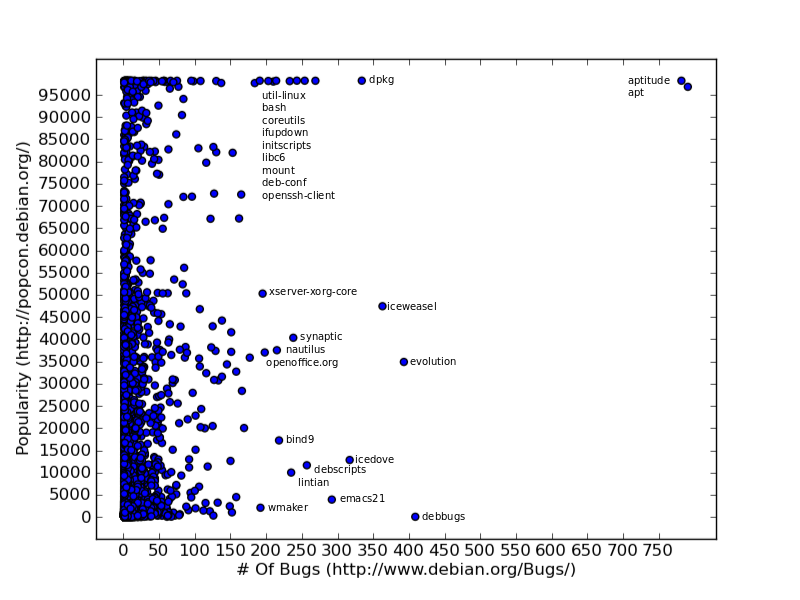
\includegraphics[width=\textwidth]{simulationpics/bugsvspopularity}
  \caption[Bugs v.s. Popularity]{A plot of the bugs a package has compared to its popularity, with notable outliers labeled}
  \label{bugsvspop}
\end{center}
\end{figure}

The first thing to note is that there seems to be very little relationship between the two variables, other than the package with the most bug reports is also one of the most used components.
The second thing to note is that the packages with the largest amount of bugs are ``apt'' and ``aptitude'' the two most popular package managers.
This could be because those packages are very buggy, or it could be because problems caused by apt, e.g. trying and failing to install a faulty package, may be reported as a problem with apt.

The last thing to notice is that there are many less popular components that have many bug reports.
When identifying the purposes of these packages many are used by developers, e.g. emacs21 is a popular text editor to program in.
The reason for their increased amount of bug reports may be that the users have prior experience and appreciation for the bug reports and the maintenance process, so file more bugs.

Measuring a components likely hood of failure using bug reports is then hypothesised to be impractical if not impossible,
as a component purpose and a components users may affect the results of the best measurement method available.
Other methods of finding a components likelihood of failure have not been further explored since this variable was eliminated from the configuration.
Though, it is expected that this is an intractable problem that is likely impossible to simulate accurately.

\subsection{Further Validation}
The assignment of the configuration variables is a different stage in the validation of this simulation.
Clearly if you create a configuration that is completely unrealistic, the saying ``garbage in, garbage out'' applies to the results.
However, this is not a concern when validating the conceptual model, or the abstract processes.
Further discussion of the validation of the assignment of the configuration variables is in chapter \ref{ubunutsimulation}.

\section{Summary}
{}In this chapter possible options were discussed for studying various strategies employed when evolving component systems.
{}Simulation, through the methodology \cite{Law2005} describes, was selected, and the steps involved were described.
{}The central artifact of this methodology, the conceptual model, was broken down into models of the user, repository and solver, and the processes of simulation.
{}These models were validated through regular meetings with the core stakeholders, and a survey conducted on subject matter experts.
{}In the next chapter the configuration of the simulation is further defined, and the questions about component system evolution are attempted to be answered.
